\documentclass[letterpaper, 11pt]{article}
%\usepackage{amsmath}
\usepackage{mathtools}
\usepackage{amssymb, amsthm}
\usepackage{tikz}
\usepackage{tkz-graph}
\usetikzlibrary{arrows,automata}
\usepackage[nointegrals]{wasysym}
%\usepackage{graphicx}

\newcommand{\red}[1]{\textcolor{red}{#1}}

\parskip=\medskipamount \parindent=0pt

\newtheorem{theorem}{Theorem}
\newtheorem{lemma}[theorem]{Lemma}
\newtheorem{proposition}[theorem]{Proposition}
\newtheorem{corollary}[theorem]{Corollary}

\theoremstyle{definition}
\newtheorem{definition}[theorem]{Definition}
\newtheorem{hypothesis}[theorem]{Hypothesis}
\newtheorem{problem}[theorem]{Problem}
\newtheorem{example}[theorem]{Example}
\newtheorem{exercise}[theorem]{Exercise}
\newtheorem{remark}{Remark}
\newtheorem{algorithm}[remark]{Algorithm}

\begin{document}

\centerline{\LARGE\bf Ma 236 Notes - Spring 2019}

\tableofcontents

\newpage


These notes are an outline of topics covered in the first part of Ma 236. For more information you should consult the text or Schaum's Outline of Logic.

\section{Propositional Logic}

{\bf References:} Chapter 1 of the text and Chapter 3.1-3.6 of Schaum's Outline

\subsection{Valid arguments}

An argument is {\em valid} if its conclusion is true whenever all its premises are. The following argument is valid. 

\begin{center}
\begin{tabular}{lc}
Premise 1:	& Min is not both home and on board\\
Premise 2:	& She's home\\ \hline
\rule{0pt}{12pt}Conclusion:	& She's not on board
\end{tabular}
\end{center}

We analyze this argument by first converting it to symbolic form. Let $H$ stand for ``Min is home'' and $B$ for ``Min is on board''. Our argument becomes

\begin{center}
\begin{tabular}{lc}
Premise 1:	& Not ($H$ and $B$)\\
Premise 2:	& $H$\\ \hline
\rule{0pt}{12pt}Conclusion:	& Not $B$
\end{tabular}
\end{center}

Next use a truth table to check the truth values of the premises and the conclusion for all possible combinations of truth values for $H$ and $B$.
\begin{center}
\begin{tabular}{cc|lccc}
 $H$ & $B$ & Not  ($H$ and $B$) & $H$ & Not $B$ \\\hline
 t & t & \quad\red{f}\quad\quad ( t ) &\red{t} &\red{f}\\
 t & f & \quad\red{t}\quad\quad ( f ) &\red{t} &\red{t}\\
 f & t & \quad\red{t}\quad\quad ( f ) &\red{f} &\red{f}\\
 f & f & \quad\red{t}\quad\quad ( f ) &\red{f} &\red{t}
\end{tabular}\\
A truth table. Truth values of premises and conclusion are \red{red}.
\end{center}
There is one row for each choice of truth values for $H$ and $B$. Since no row has $\textcolor{red}{t\,t\, f}$, the argument is valid. 

Notice that whether or not the premises are true in real life does not affect whether or not the argument is valid. 

\subsubsection{Sound arguments}

A valid argument in which all premises are true in real life is called {\em sound}. The conclusion of a sound argument is true in real life. 

\subsection{An invalid argument}

The following argument is not valid.

\begin{center}
\begin{tabular}{lc}
Premise 1:	& Min is home or on board\\
Premise 2:	& She's home\\ \hline
\rule{0pt}{12pt}Conclusion:	& She's not on board
\end{tabular}
\end{center}

To test validity keep $H$ and $B$ as before and convert to symbolic form:

\begin{center}
\begin{tabular}{lc}
Premise 1:	& $H \vee B$\\
Premise 2:	& $H$\\ \hline
\rule{0pt}{12pt}Conclusion:	& $\neg B$
\end{tabular}
\end{center}

{\bf New notation:} Write $\vee$ for ``or'' and $\neg$\, for ``not''. Likewise $\wedge$ for ``and''.

``Or'' is ambiguous. It can mean ``one or the other or both'', but it can also mean ``one or the other but not both''.  The symbol $\vee$ carries the first meaning. 

The argument above is not valid because there is a counterexample.

\begin{center}
\begin{tabular}{cc|ccc}
 $H$ & $B$ & $H\vee B$ & $H$ & $\neg B$ \\\hline
 t & t &  t  & t & f\\
 t & f &  t  & t & t\\
 f & t &  t  & f & f\\
 f & f &  f  & f & t
\end{tabular}\\
The first row is a counterexample.
\end{center}

\subsection{Sentences}

\subsubsection{Atomic sentences}

Simple English sentences which are either true or false are represented symbolically by capital letters. For example

\begin{itemize}
\item [$A:$] Frogs have feathers. 
\item [$B:$] It will rain tomorrow. 
\item [$C:$] He is a college student.
\end{itemize}

Some English sentences are neither true nor false:

\begin{itemize}
\item Please put away your cell phones.
\item What is the point of this course?
\end{itemize}

\subsubsection{Compound sentences}

More complicated English sentences are represented symbolically by using $\neg, \vee, \wedge$. For example

\begin{quote}
Either it will rain tomorrow and he is a college student, or it will not rain tomorrow and frogs have feathers.
\end{quote}

may be translated as $(B\wedge C) \vee (\neg B \wedge A)$.

\subsubsection{Logical equivalence}

Every symbolic sentence has a truth table. Two sentences with the same truth table are {\em logically equivalent}.


\subsubsection{Rules of formation}

Symbolic sentences are often called propositions. We will call them just sentences for short. 
 
\begin{enumerate}
\item Letters $A, B, C,\ldots$ with or without subscripts are sentences.
\item If $\square$ is any sentence, so is $\neg\, \square$.
\item If $\square$ and $\triangle$ are sentences, so are $(\square\vee \triangle)$ and $(\square\wedge \triangle)$. More generally if $\square_1,\ldots, \square_n$ are sentences, so are $(\square_1\vee \cdots \vee \square_n)$ and $(\square_1\wedge \cdots \wedge \square_n)$
\end{enumerate}

Using these rules we can show formally that $(B\wedge C) \vee (\neg B \wedge A)$ is a sentence.

\begin{tabular}{lll}
1. &$A$, $B$, and $C$ are sentences & By Rule 1\\
2. &$\neg B$ is a sentence & From Step 1 and Rule 2\\
3. &$(B\wedge C)$ and $(\neg B \wedge A)$ are sentences & Steps 1,2 and Rule 3\\
4. &$((B\wedge C)\vee(\neg B \wedge A))$ is a sentences & Step 3 and Rule 3\\
\end{tabular}

Strictly speaking  $(B\wedge C) \vee (\neg B \wedge A)$ is not correctly formed; it is missing its outer parentheses. For convenience we allow ourselves to leave off the outer parentheses when it does not cause confusion.

\subsection{Conditionals}

\subsubsection{$\to$}

We agree that the following argument is valid. 

\begin{center}
\begin{tabular}{cc}
If Min works on board that tub, she is underpaid &If $W$, then $U$\\
She works on board that tub &$W$\\\hline
\rule{0pt}{12pt}She is underpaid & $U$
\end{tabular}
\end{center}

When $W$ is true, and $U$ is false, then ``If $W$, then $U$'' must be false or else the argument would not be valid. Thus we know Line 2 in the following truth table.

{\bf New notation.} Write ``If $W$, then $U$'' symbolically as ``$W\to U$''.

\smallskip
\centerline{
\begin{tabular}{cc|c}
 $W$ & $U$ &  $W\to U$ \\\hline
 t & t & t\\
 t & f & f\\
 f & t & t\\
 f & f & t 
\end{tabular}}

The other lines may seem strange, because in ordinary conversation we would say ``If Min works on board that tub, she is underpaid'' we know for a fact that she does not work on that tub or we know for a fact that she is underpaid. 

$W\to U$ is logically equivalent to $\neg W\vee U$ (as you can easily check).

$\to$ has many translations into English: $A$:Min is home; $C$:Hen is home.
\centerline{\begin{tabular}{lll}
If Min is home, then Hen is 	&If $A$ then $C$	&$A\to C$\\
If Min is home, Hen is		&If $A$, $C$		&$A\to C$\\
Hen is home if Min is		&$C$ if $A$		&$A\to C$\\
Min is home only if Hen is	&$A$ only if $C$	&$A\to C$\\
Only if Hen is home is Min home&Only if $C$, $A$	&$A\to C$
\end{tabular}}

``Only if'' can be confusing. Think of it this way: ``Min is home only if Hen is'' is equivalent to ``Min cannot be home if Hen is not home'', i.e. $\neg C \to \neg A$. But $\neg C \to \neg A$ is logically equivalent to $A\to C$ (as you can check).

Is the following argument valid? If not, find a counterexample.
\begin{quote}
Look, we know that Min is on board if Henry is home. Then she has to be on board if she's home, because Henry is home if she is.
\end{quote}

$A$:Henry is home \quad $B$:Min is on board \quad $C$:Min is home.

\begin{center}
\begin{tabular}{cc}
Min is on board if Henry is home &  $A\to B$\\
Henry is home if she is &$ C\to A$\\\hline
\rule{0pt}{12pt}She has to be on board if she's home. & $C\to B$
\end{tabular}
\end{center}


\subsubsection{$\leftrightarrow$}


$A$ if and only if $C$ is written symbolically as $A\leftrightarrow C$.

\smallskip
\centerline{\begin{tabular}{cc|c}
 $A$ & $C$ &  $A\leftrightarrow C$  \\\hline
 t   & t   &        t \\
 t   & f   &        f	\\
 f   & t   &        f \\
 f   & f   &        t     
\end{tabular}}

$A\leftrightarrow C$ is logically equivalent to $(A\to C) \wedge (C\to A)$.

\subsection{Translation}

$A\to B$ is logically equivalent to $\neg(A\wedge \neg B)$ and also to $\neg A \vee B$, but these equivalences do not seem to hold up in everyday language.

\begin{tabular}{ll}
Socrates is dead & $B$ \\ \hline
\rule{0pt}{12pt} If George sits down, then Socrates is dead & $A \to B$
\end{tabular}

\begin{tabular}{ll}
It's not the case that if I break my leg today, I'll ski tomorrow & $\neg (A\to B)$ \\ \hline
\rule{0pt}{12pt} I'll break my leg today & $A$
\end{tabular}

\begin{tabular}{ll}
If they withdraw if we advance, we'll win & $(A\to B)\to C$ \\ 
We won't advance & $\neg A$\\\hline
\rule{0pt}{12pt} We'll win & $C$
\end{tabular}

\subsection{Complete rules of formation}\label{se:complete}

\begin{enumerate}
\item Capital letters are sentences: $A, B, \ldots, A_1, A_2,\ldots$.
\item If $\square$ is a sentence, so is $\neg \square$.
\item If $\square_1,\ldots, \square_n$, $n\ge 2$, are sentences, so are $(\square_1\wedge \square_2\wedge \cdots \wedge \square_n)$ and $(\square_1\vee \square_2 \vee \cdots \vee \square_n)$
\item If $\square$ and $\triangle$ are sentences, so are $(\square \to \triangle)$ and $(\square \leftrightarrow\triangle)$.
\item Nothing else is a sentence (until the next chapter).
\end{enumerate}


\subsection{Tautologies}

A tautology is a sentence which is always true. For example $A\vee \neg A$.

The sentence $\square$ is a tautology if and only if the argument (with no premises)
\ \begin{tabular}{l}
\\\hline
\rule{0pt}{12pt}
$\square$
\end{tabular}\ 
is valid. 



\newpage
\section{Refutation Trees}



{\bf References:} Chapter 2 of the text and Chapter 3.7 of Schaum's Outline

To test if a sentence $\alpha$ is a tautology, we can use truth tables to check that if $\alpha$ is always true. Or we can use truth tables to check if $\neg \alpha$ is never true. In this chapter we introduce a more efficient way to check if a sentence is never true.

We use refutation trees (called truth trees in the text) to decide whether or not a sentence is never true. In fact using refutation trees we can decide if a bunch of sentences are never all true at the same time.

\begin{definition} A set of sentences {\em consistent} if the sentences can all be true at the same time. The set is {\em inconsistent} if the sentences are never all true at the same time.
\end{definition}

\subsection{A closed tree}

Use the tree method to test the sentences {$B\to\neg A$}, {$\neg B \to C$} and {$\neg(A\to C)$} for consistency.

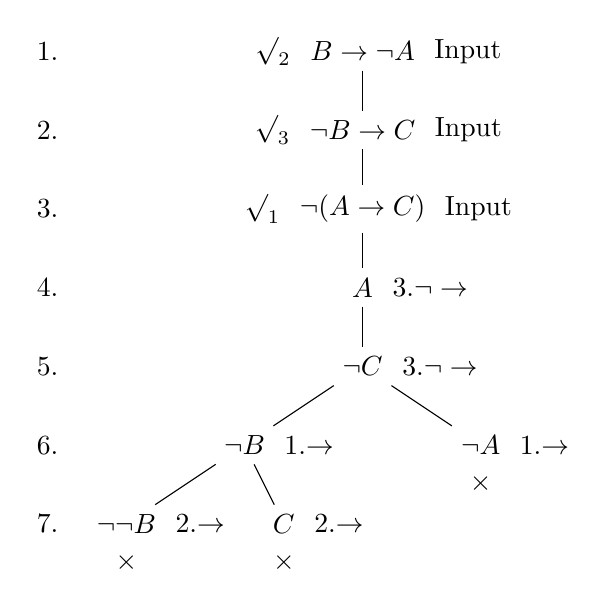
\begin{tikzpicture}
\draw (0,0)      node (11)                       {1.};
\draw (4cm,0)    node (13) [label=left:$\surd_2$][label=right:Input] {$B\to\neg A$};

\draw (0,-1cm)   node (21)                      {2.};
\draw (4cm,-1cm) node (23) [label=left:$\surd_3$][label=right:Input] {$\neg B \to C$};
\draw (13) -- (23);

\draw (0,-2cm)   node (31)                      {3.};
\draw (4cm,-2cm) node (33) [label=left:$\surd_1$] [label=right:Input]{$\neg(A\to C)$};
\draw (23) -- (33);

\draw (0,-3cm)   node (41) {4.};
\draw (4cm,-3cm) node (43)  [label=right: 3.$\neg\to$]  {$A$};
\draw (33) -- (43);

\draw (0,-4cm)   node (51)                      {5.};
\draw (4cm,-4cm) node (53)  [label=right: 3.$\neg\to$] {$\neg C$};
\draw (43) -- (53);

\draw (0,-5cm)   node (61)                      {6.};
\draw (2.5cm,-5cm) node (62)  [label=right:1.$\to$]  {$\neg B$}; 
\draw (5.5cm,-5cm)  node (64)  [label=right:1.$\to$] [label=below:$\times$] {$\neg A$};
\draw (53)--(62);
\draw (53)--(64);

\draw (0, -6cm) node (71)                       {7.};
\draw (1cm,-6cm) node (72) [label=right:2.$\to$] [label=below:$\times$]{$\neg\neg B$};
\draw (3cm,-6cm) node (73)  [label=right:2.$\to$] [label=below:$\times$]{$C$};
\draw (62)--(72);
\draw (62)--(73);
\end{tikzpicture}

After each step put $\times$ at the bottom of every path which contains a sentence and its negation; there is no way all the sentences in such a path can be true at the same time. 

The tree test is finished when there are no more rules to apply. In the present case all paths close, so the sentences are inconsistent. The subscripts on the $\surd$'s show the order in the rules of inference were applied. If the rules are applied in a different order, the resulting trees will be different, but all paths will still close.

\subsection{A tree which does not close}

Use the tree test to see if the sentences $A\to B$, $\neg A$ and $\neg B$ are consistent.

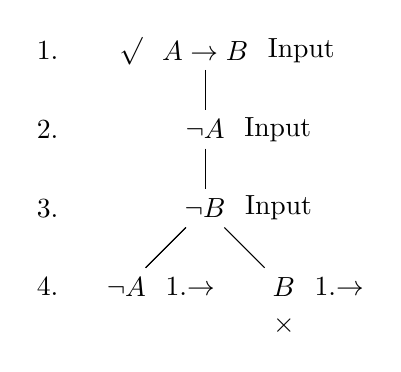
\begin{tikzpicture}
\draw (0,0)      node (11)                       {1.};
\draw (2cm,0)    node (13) [label=left:$\surd$][label=right:Input] {$A\to B$};

\draw (0,-1cm)   node (21)                      {2.};
\draw (2cm,-1cm) node (23) [label=right:Input] {$\neg A$};
\draw (13) -- (23);

\draw (0,-2cm)   node (31)                      {3.};
\draw (2cm,-2cm) node (33) [label=right:Input]{$\neg B$};
\draw (23) -- (33);

\draw (0,-3cm)   node (41) {4.};
\draw (1cm,-3cm) node (43)  [label=right: 1.$\to$]  {$\neg A$};
\draw (33) -- (43);
\draw (3cm,-3cm) node (45)  [label=right: 1.$\to$][label=below:$\times$]  {$B$};
\draw (33) -- (43);
\draw (33) -- (45);
\end{tikzpicture}

We are done after just one step. There is an open path, so the sentences  $A\to B$, $\neg A$ and $\neg B$ are consistent. Truth values which make all the sentences true may be read off from any open path.

\subsection{Rules of inference (preliminary version)}

{\small
\[\begin{tabular}{|c|c|c|c|c|}
\hline
\begin{tabular}{c}
\rule{0pt}{15pt}
$\square$\\
\hspace{-6pt}$\neg\, \square$\\ \hline
$\rule{0pt}{12pt}\times$
\end{tabular}
&
\begin{tabular}{c}
$\surd (\square\to\triangle)$\\ \hline
$\rule{0pt}{12pt}\neg\square \quad\quad \triangle$
\end{tabular}
&
\begin{tabular}{c}
$\surd (\square\leftrightarrow\triangle)$\\ \hline
$\rule{0pt}{12pt}\square \quad\quad  \neg\,\square$\\
$\rule{0pt}{12pt}\triangle \quad\quad  \neg\triangle$
\end{tabular}
&
\begin{tabular}{c}
$\surd (\square\vee\triangle)$\\ \hline
$\rule{0pt}{12pt}\square \quad\quad \triangle$
\end{tabular}
&
\begin{tabular}{c}
$\surd (\square\wedge\triangle)$\\ \hline
$\rule{0pt}{12pt}\square$\\
$\rule{0pt}{12pt}\triangle$\\
\end{tabular}
\\\hline %*************************************************
\begin{tabular}{c}
$\surd\ \neg \neg \square$\\ \hline
$\rule{0pt}{12pt}\square$
\end{tabular}
&
\begin{tabular}{c}
\rule{0pt}{15pt}$\surd \neg\,(\square\to\triangle)$\\ \hline
$\rule{0pt}{12pt}\square$\\
$\hspace{-9pt}\neg\,\triangle$
\end{tabular}
&
\begin{tabular}{c}
$\surd \neg\,(\square\leftrightarrow\triangle)$\\ \hline
$\rule{0pt}{12pt}\neg\,\square \quad\quad \square$\\
$\rule{0pt}{12pt}\hspace{7pt}\triangle \hspace{14pt} \neg\,\triangle$\\
\end{tabular}
&
\begin{tabular}{c}
$\surd \neg\,(\square\vee\triangle)$\\ \hline
$\rule{0pt}{12pt}\neg\,\square$\\$\neg\,\triangle$
\end{tabular}
&
\begin{tabular}{c}
$\surd \neg\,(\square\wedge\triangle)$\\ \hline
$\rule{0pt}{12pt}\neg\,\square \quad\quad\neg\,\triangle$\\
\end{tabular}\\\hline

\end{tabular}\]

\[\begin{tabular}{|c|c|c|c|c|}
\hline
\begin{tabular}{c}
$\surd (\square\vee\triangle\vee\Circle)$\\ \hline
$\rule{0pt}{12pt}\square \quad\quad \triangle \quad\quad\Circle$
\end{tabular}
&
\begin{tabular}{c}
$\surd (\square\wedge\triangle\wedge\Circle)$\\ \hline
$\rule{0pt}{12pt}\square$\\
$\rule{0pt}{12pt}\triangle$\\
$\rule{0pt}{12pt}\Circle$\\
\end{tabular}
\\\hline %*************************************************
\begin{tabular}{c}
$\surd \neg\,(\square\vee\triangle\vee\Circle)$\\ \hline
$\rule{0pt}{12pt}\neg\,\square$\\$\neg\,\triangle$\\$\neg\,\Circle$
\end{tabular}
&
\begin{tabular}{c}
$\surd \neg\,(\square\wedge\triangle\wedge\Circle)$\\ \hline
$\rule{0pt}{12pt}\neg\,\square\quad\quad\neg\,\triangle\quad\quad\neg\,\Circle$\\
\end{tabular}\\\hline

\end{tabular}\]
}

\subsection{Exercises}

\begin{enumerate}
 \item Interpret ``E'', ``J'' and ``M'' as meaning that the earth is the third planet from the sun, that Jupiter is, and that Mars is. Work out the truth values (in real life) of the following sentences.

\begin{tabular}{ll}
(a) $(M\wedge J) \vee E$	& (b) $M\wedge (J \vee E)$ \\
(c) $\neg(M \vee J \vee E)$	& (d) $\neg M \vee J \vee E$ \\
(e) $\neg(\neg M \vee \neg J \vee \neg E)$ & (f) $\neg(\neg M \wedge \neg J \wedge \neg E)$
\end{tabular}

\item ``Thin is guilty,'' observed Watson,``because (i) either Holmes is right and the vile Moriarty is guilty or he is wrong and the scurrilous Thin did the job; but (ii) those scoundrels are either both guilty or both innocent; and, as usual, (iii) Holmes is right.''

(a) Write down the argument symbolically. Use ``$T, M$'' for ``Thin is guilty, Moriarty is guilty'', ``$\neg T,\neg M$'' for innocence, and ``$H$'' for ``Holmes is right.''

(b) Is the argument valid? 
 
(c) Are the premises and the conclusion consistent, i.e., is there a case in which they are all true?

 Solve (b) and (c) efficiently by looking for counterexamples and then solve them by truth tables.

\item \parbox{3.5in}{Use a truth tree to show that this argument is valid.}\quad
\begin{tabular}{l}
$A\vee B$\\
$A\to C$\\
$B\to C$\\\hline
$C$
\end{tabular}

\item Convert the following arguments to symbolic notation, and then use truth trees to check if they are valid. Find a counterexample for each argument which is not valid.
\begin{enumerate}
\item Moriarty: ``If Min is home, so is Henry.'' Thin: ``Indeed, and if Min is home, Henry isn't.'' Moriarty: ``Ah, I see. Min's not home.''
\item ``Min's home if Henry is, but he isn't, so she isn't.''
\item ``It's false that if Min is home, she's on board. Then if she's home, she's not on board.''
\item ``It's false that if Min is home, she's on board, because if she's home, she's not on board.''
\item ``Look, we know that Min is on board if Henry is home. Then she has to be on board if she's home, because Henry's home if she is.''
\end{enumerate}

\end{enumerate}

\newpage
\section{Predicate Logic}

{\bf References:} Chapter 3 of the text and Chapter 6 of Schaum's Outline

\subsection{The tree test for sentences with quantifiers}

\begin{tabular}{ll}
{ A valid argument:}&
\begin{tabular}{ll}
Everyone can trap Moriarty & $\forall x\, Txb$\\\hline
Watson can trap Moriarty  &  $Tab$ 
\end{tabular}\\
\\
{ An invalid argument:}&
\begin{tabular}{ll}
Someone can trap Moriarty & $\exists x\, Txb$\\\hline
Watson can trap Moriarty  &  $Tab$ 
\end{tabular}\\
\\
{ New notation:}&\framebox{
\begin{tabular}{ll}
$\forall x$  & for all $x$\\
$\exists x$  & for some $x$\\
 $a$         & Watson\\
 $b$         & Moriarty\\
 $Txy$    & $x$ can trap $y$\\
 $x$, $y$    & variables    
\end{tabular}}
\end{tabular}\\

An argument is valid if and only if the premises and the negation of the conclusion are {\em inconsistent}. Thus we can use the tree test to check if the arguments above are valid, but we need some additional rules of inference.


\subsubsection{Rules of inference for $\mathbf \neg$}

\[\begin{tabular}{|c|c|c|c|}
\hline
\begin{tabular}{r}
$\surd\, \neg\forall\,\square$\\ \hline
$\rule{0pt}{12pt}\exists \neg\,\square$
\end{tabular}
&
\begin{tabular}{r}
$\surd\, \neg\exists\,\square$\\ \hline
$\rule{0pt}{12pt}\forall \neg\,\square$
\end{tabular}
&
\begin{tabular}{r}
$\surd \neg\,\neg\,\square$\\ \hline
$\rule{0pt}{12pt}\square$
\end{tabular}
&
\begin{tabular}{r}
\rule{0pt}{15pt}
$\square$\\
\hspace{-6pt}$\neg\, \square$\\ \hline
$\rule{0pt}{12pt}\times$
\end{tabular}\\\hline

\end{tabular}\]

\subsubsection{Rules of inference for $\mathbf \to, \leftrightarrow, \vee, \wedge$}

\[\begin{tabular}{|c|c|c|c|}
\hline
\begin{tabular}{c}
$\surd (\square\to\triangle)$\\ \hline
$\rule{0pt}{12pt}\neg\square \quad\quad \triangle$
\end{tabular}
&
\begin{tabular}{c}
$\surd (\square\leftrightarrow\triangle)$\\ \hline
$\rule{0pt}{12pt}\square \quad\quad  \neg\,\square$\\
$\rule{0pt}{12pt}\triangle \quad\quad  \neg\triangle$
\end{tabular}
&
\begin{tabular}{c}
$\surd (\square\vee\triangle)$\\ \hline
$\rule{0pt}{12pt}\square \quad\quad \triangle$
\end{tabular}
&
\begin{tabular}{c}
$\surd (\square\wedge\triangle)$\\ \hline
$\rule{0pt}{12pt}\square$\\
$\rule{0pt}{12pt}\triangle$\\
\end{tabular}
\\\hline %*************************************************
\begin{tabular}{c}
\rule{0pt}{15pt}$\surd \neg\,(\square\to\triangle)$\\ \hline
$\rule{0pt}{12pt}\square$\\
$\hspace{-9pt}\neg\,\triangle$
\end{tabular}
&
\begin{tabular}{c}
$\surd \neg\,(\square\leftrightarrow\triangle)$\\ \hline
$\rule{0pt}{12pt}\neg\,\square \quad\quad \square$\\
$\rule{0pt}{12pt}\hspace{7pt}\triangle \hspace{14pt} \neg\,\triangle$\\
\end{tabular}
&
\begin{tabular}{c}
$\surd \neg\,(\square\vee\triangle)$\\ \hline
$\rule{0pt}{12pt}\neg\,\square$\\$\neg\,\triangle$
\end{tabular}
&
\begin{tabular}{c}
$\surd \neg\,(\square\wedge\triangle)$\\ \hline
$\rule{0pt}{12pt}\neg\,\square \quad\quad\neg\,\triangle$\\
\end{tabular}\\\hline
\end{tabular}\]

\subsubsection{Rules of inference for $\forall$ and $\exists$}

{\bf Universal Instantiation Rule.} If an open path has a line $\forall x \ldots x \ldots$, do not check ($\surd$) this line, but add as many new lines as necessary so that for every name $n$ in the path there is a line $\ldots n \ldots$. If there are no names in the path, choose a new name $n$ and add a line $\ldots n \ldots$. 

\begin{center}
\begin{tabular}{ll}
Everyone can trap Moriarty & $\forall x\, Txb$\\\hline
Watson can trap Moriarty  &  $Tab$ 
\end{tabular}\quad
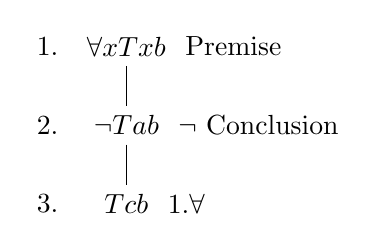
\begin{tikzpicture} [baseline=-.5in]
\draw (0,0)      node (11)                       {1.};
\draw (1cm,0)    node (13) [label=right:Premise] {$\forall x Txb$};
\draw (0,-1cm)   node (21)                      {2.};
\draw (1cm,-1cm) node (23) [label=right:$\neg$ Conclusion] {$\neg Tab$};
\draw (13) -- (23);
\draw (0,-2cm)   node (31)                      {3.};
\draw (1cm,-2cm) node (33) [label=right:1.$\forall$] {$Tcb$};
\draw (23) -- (33);
\end{tikzpicture}
\end{center}
Line~3 comes from applying the Universal Instantiation Rule to Line~1. Notice that Line 1 is not checked ($\surd)$ because we may want to use it again. Strictly speaking we should use it to add lines with $Taa$, $Tba$ and $Tbb$ to the tree, but we don't need those lines because the tree closes with just $Tab$.

{\bf Existential Instantiation Rule.} If an open path has a line $\exists x \ldots x \ldots$, check this line ($\surd$). If there are no lines $\ldots n \ldots$ in the path, choose a {\em new name} $n$, and add a line $\ldots n \ldots$.

\begin{tabular}{ll}
Someone can trap Moriarty & $\exists x\, Txb$\\\hline
Watson can trap Moriarty  &  $Tab$ 
\end{tabular}\quad
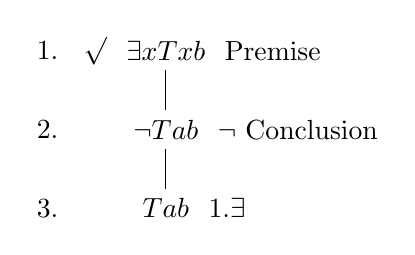
\begin{tikzpicture} [baseline=-.5in]
\draw (0,0)      node (11)                       {1.};
\draw (1.5cm,0)    node (13) [label=left:$\surd$] [label=right:Premise] {$\exists x Txb$};

\draw (0,-1cm)   node (21)                      {2.};
\draw (1.5cm,-1cm) node (23) [label=right:$\neg$ Conclusion] {$\neg Tab$};
\draw (13) -- (23);

\draw (0,-2cm)   node (31)                      {3.};
\draw (1.5cm,-2cm) node (33) [label=right:1.$\exists$]{$Tab$};
\draw (23) -- (33);
\end{tikzpicture}

The argument is invalid because there is an unclosed path. 

\subsection{Examples}

\begin{enumerate}
\item Alma paints so someone paints.

\begin{tabular}{ll}
Alma paints & $Pa$\\\hline
Someone paints & $\exists x\,Px$ 
\end{tabular}\quad
\quad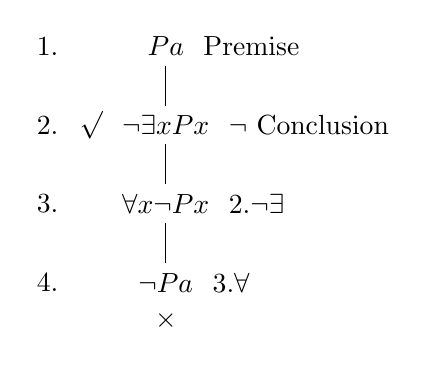
\begin{tikzpicture} [baseline=-.5in]
\draw (0,0)      node (11)                       {1.};
\draw (1.5cm,0)  node (13) [label=right:Premise] {$Pa$};

\draw (0,-1cm)   node (21)                      {2.};
\draw (1.5cm,-1cm) node (23) [label=right:$\neg$ Conclusion] [label=left:$\surd$] {$\neg \exists x Px$};
\draw (13) -- (23);

\draw (0,-2cm)   node (31)                      {3.};
\draw (1.5cm,-2cm) node (33) [label=right:2.$\neg\exists$]{$\forall x \neg Px$};
\draw (23) -- (33);

\draw (0,-3cm)   node (41)                      {4.};
\draw (1.5cm,-3cm) node (43)[label=below:$\times$] [label=right:3.$\forall$] {$\neg Pa$};
\draw (33) -- (43);
\end{tikzpicture}

\item 
Someone sings so someone paints, because all singers paint.

\begin{tabular}{ll}
Someone sings &$\exists x Sx$\\
All singers paint &$\forall x (Sx \to Px)$\\\hline
Someone paints & $\exists x\,Px$ 
\end{tabular}\quad

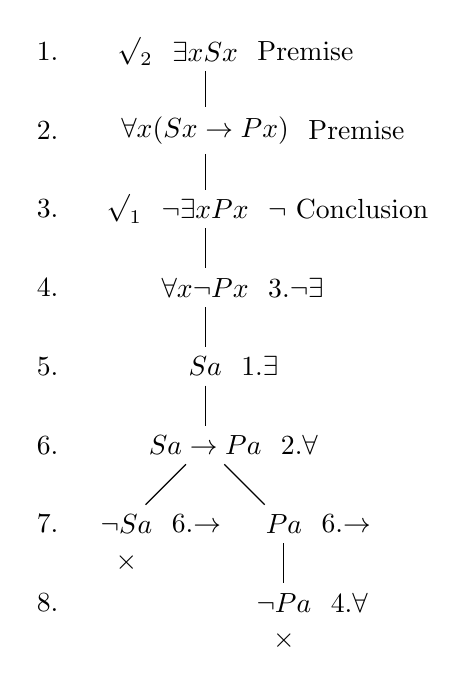
\begin{tikzpicture}
\draw (0,0)      node (11)                       {1.};
\draw (2cm,0)    node (13) [label=left:$\surd_2$][label=right:Premise] {$\exists x Sx$};

\draw (0,-1cm)   node (21)                      {2.};
\draw (2cm,-1cm) node (23) [label=right:Premise] {$\forall x (Sx \to Px)$};
\draw (13) -- (23);

\draw (0,-2cm)   node (31)                      {3.};
\draw (2cm,-2cm) node (33) [label=left:$\surd_1$] [label=right:$\neg$ Conclusion]{$\neg\exists x Px$};
\draw (23) -- (33);

\draw (0,-3cm)   node (41) {4.};
\draw (2cm,-3cm) node (43)  [label=right: 3.$\neg\exists$]  {$\forall x \neg Px$};
\draw (33) -- (43);

\draw (0,-4cm)   node (51)                      {5.};
\draw (2cm,-4cm) node (53)  [label=right: 1.$\exists$] {$Sa$};
\draw (43) -- (53);

\draw (0,-5cm)   node (61)                      {6.};
\draw (2cm,-5cm) node (63)  [label=right: 2.$\forall$] {$Sa\to Pa$};
\draw (53) -- (63);

\draw (0,-6cm)   node (71)                      {7.};
\draw (1cm,-6cm) node (72)  [label=right:6.$\to$] [label=below:$\times$] {$\neg Sa$}; 
\draw (3cm,-6cm)  node (74)  [label=right:6.$\to$]  {$Pa$};
\draw (63)--(72);
\draw (63)--(74);

\draw (0, -7cm) node (81)                       {8.};
\draw (3cm,-7cm) node (82) [label=right:4.$\forall$] [label=below:$\times$]{$\neg Pa$};
\draw (74)--(82);
\end{tikzpicture}

\item Construct a refutation tree to decide if the following argument is valid. Justify each line in the tree. 

\begin{tabular}{l}
$\forall x \forall y (Lxy \to Lyx)$\\
$\exists x Lax$\\\hline
$\exists x Lxa$
\end{tabular}

An answer is on the next page, but try the problem before you look.  (There is more than one answer depending on the order in which you apply the rules of inference.)

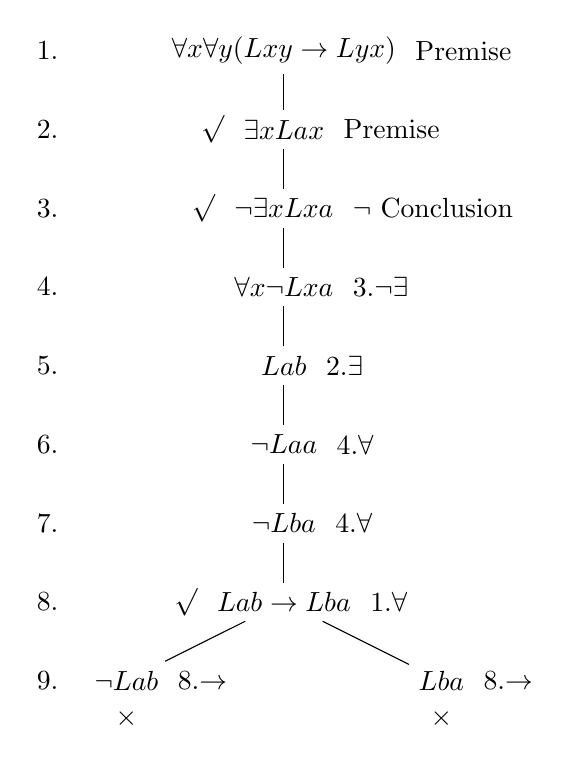
\begin{tikzpicture}[baseline=-.5in]
\draw (0,0)     node (11)                       {1.};
\draw (3cm,0)   node (13) [label=right:Premise] {$\forall x\forall y (Lxy\to Lyx)$};

\draw (0,-1cm)   node (21)                      {2.};
\draw (3cm,-1cm) node (23) [label=left:$\surd$] [label=right:Premise] {$\exists x Lax$};
\draw (13) -- (23);

\draw (0,-2cm)   node (31)                      {3.};
\draw (3cm,-2cm) node (33) [label=left:$\surd$][label=right:$\neg$ Conclusion]  {$\neg\exists x Lxa$}; 
\draw (23) -- (33);

\draw (0cm,-3cm) node (41)                    {4.};
\draw (3cm,-3cm) node (43) [label=right:3.$\neg \exists$] {$\forall x \neg Lxa$};                    
\draw (33) -- (43);

\draw (0,-4cm)   node (51)                    {5.};
\draw (3cm,-4cm) node (53) [label=right:2.$\exists$]    {$Lab$}; 
\draw (43) -- (53);

\draw (0,-5cm)   node (61)                      {6.};
\draw (3cm,-5cm) node (63)  [label=right:4.$\forall$]  {$\neg Laa$};
\draw (53) -- (63);

\draw (0,-6cm)   node (71)                      {7.};
\draw (3cm,-6cm) node (73)  [label=right:4.$\forall$] {$\neg Lba$};
\draw (63) -- (73);

\draw (0,-7cm)   node (81)                      {8.};
\draw (3cm,-7cm) node (83)   [label=left:$\surd$]  [label=right:1.$\forall$]  {$Lab \to  Lba$}; 
\draw (73) -- (83);

\draw (0,-8cm)   node (91)                      {9.};
\draw (1cm,-8cm) node (92)  [label=right:8.$\to$] [label=below:$\times$]  {$\neg Lab$};
\draw (5cm,-8cm) node (94)  [label=right:8.$\to$] [label=below:$\times$] {$Lba$};
\draw (83) -- (92);
\draw (83) -- (94);
\end{tikzpicture}

This argument is valid because all paths close. Since all paths close, it is not necessary to do all applications of the $\forall$ rule to line 1. In other words you do not need to add lines $Laa \to  Laa$, $Lba \to  Lab$ and $Lbb \to  Lbb$ to the tree.

If there were an open path you would need all these lines. First because they might close the open path; and second because even if they do not, they ensure that the first premise is true in the counterexample corresponding to the open path.  

In general as long as all paths close, the rules of inference may be applied in any order. 

\end{enumerate}

\subsection{Identity}

The identity predicate $Ixy$ is always interpreted as equality. $Ixy$ is true if and only if $x$ and $y$ are equal. That being the case, we write $x=y$ instead of $Ixy$ and $x\neq y$ or $\neg x=y$ instead of $\neg Ixy$.

\begin{example} ``There are at most 2 things'' can be translated into symbolic form as
\[\exists x \exists y \forall z\, z=x \vee z=y.\]
\end{example}

\begin{exercise} Translate 
\begin{enumerate} 
\item ``There are at most 3 things''.
\item ``There are at least 2 things''
\item ``There are exactly 2 things''
\end{enumerate}
\end{exercise}

The rules of inference for $=$ are as follows. \\

\centerline{
\begin{tabular}{c}
$a\neq a$\\ \hline
$\rule{0pt}{12pt}\times$
\end{tabular}\quad\quad\quad
\begin{tabular}{c}
$a = b$\\ 
$\ldots a \ldots$\\
\hline
$\ldots b\ldots$
\end{tabular}
\quad or \quad
\begin{tabular}{c}
$a = b$\\ 
$\ldots b \ldots$\\
\hline
$\ldots a\ldots$
\end{tabular}
}

See the flowchart on page 77 of the text.

\end{document}

\section{Model Theory}

A model of a set $S$ of sentences is an interpretation in which all the sentences in $S$ are true. For example suppose $S$ is the following set with one element. 
\[ S = \{\exists x \exists y\,\forall z\, (z=x \vee z=y)\}.
\]
The models of this $S$ are just the sets with at most two elements (and no other sets).

\begin{theorem}[The Compactness Theorem]\label{th:compactness} If $S$ is a set of sentences and every finite subset of $S$ has a model, then $S$ has a model.
\end{theorem}

\subsection{Saying that there are only finitely many things}

It is clear from the example above that for each $n = 2, 3, 4, \ldots$ there is a sentence whose models are the sets with at most $n$ elements. Call this sentence $\sigma_n$.

$\sigma_n$ is a translation of ``there are at most n things'',
but we will see that there is no translation of `` there are only finitely many things''. This is what we mean when we say that finiteness is not a first order property (predicate logic is also called first order logic).

\begin{theorem}\label{th:finiteness}
There is no sentence whose models are all finite sets and no infinite sets.
\end{theorem}
\begin{proof}
Suppose $\tau$ is such a sentence. Any model of 
\[S = \{ \tau, \neg\sigma_2, \neg\sigma_3, \neg\sigma_4, \ldots\}\]   
would be an infinite model of $\{\tau\}$, so $S$ cannot have any models. 

On the other hand every finite subset $F\subset S$ does have a model. Indeed all large enough finite sets are are models of $F$. Thus by the Compactness Theorem (Theorem~\ref{th:compactness}), $S$ has a model. This contradiction shows that there cannot be any such sentence $\tau$.
\end{proof}
 
We have only mentioned the predicate $=$. If there are names and other predicates in our language, then Theorem~\ref{th:finiteness} becomes
\begin{theorem}  If a sentence $\tau$ has arbitrarily large models, then $\tau$ has an infinite model. 
\end{theorem}

\subsection{Graph theory}

A graph consists of vertices joined by edges. There is at most one edge between any two vertices.\footnote{In spite of what was said in class, we allow loops. It is too much trouble to be always excluding them.}\\

\centerline{
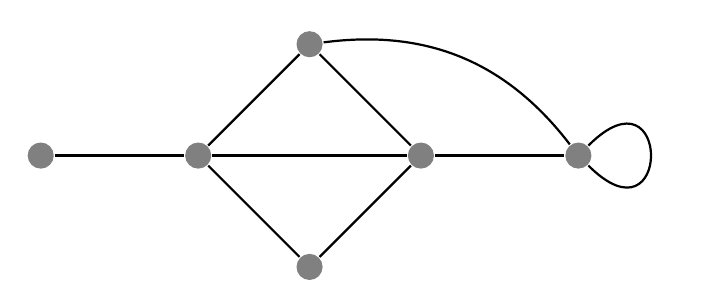
\begin{tikzpicture}[-,>=stealth',auto,node distance=2cm, thick]
  \node (A) [fill=gray, circle, minimum size=.25cm]                   {};
  \node (B) [fill=gray, circle, minimum size=.25cm, above right of=A] {};
  \node (D) [fill=gray, circle, minimum size=.25cm, below right of=A] {};
  \node (C) [fill=gray, circle, minimum size=.25cm, below right of=B] {};
  \node (E) [fill=gray, circle, minimum size=.25cm, right of=C]       {};
  \node (F) [fill=gray, circle, minimum size=.25cm, left of=A]        {};
  \path (A) edge               (B)
            edge               (C)
        (B) edge               (C)
        (C) edge               (D)
            edge               (E)
        (D) edge               (A)
        (E) edge [bend right]  (B)
            edge [distance=1.5cm, out=45,in=315] (E) 
        (F) edge               (A);
\end{tikzpicture}
}
\centerline{A graph}

To talk about graphs we use English or the language of graph theory. This language has two predicates: $\sim$ and $=$. The domain of an interpretation is a nonempty set of vertices, and the $x\sim y$ is true in an interpretation if vertices $x$ and $y$ are joined by an edge. $x=y$ is true if $x$ and $y$ are the same vertex.

\begin{example} 
The graph shown above has six vertices (the gray dots). In particular it has a vertex with a loop. ``There is a vertex with a loop'' translates into the language of graph theory as \[\exists x\, x\sim x. \]  
\end{example}

The {\em degree} of a vertex is the number of edges attached to it. A loop counts as two attached edges. 

\begin{exercise} Translate.
\begin{enumerate}
\item There is an isolated vertex (a vertex of degree 0).
\item There is a vertex of degree 1.
\item All vertices have degree at most 2.
\item $\forall x \forall y\, x=y$.
\item $\exists x \exists y \forall z\, (x\sim z \leftrightarrow z=y)$.
\end{enumerate}
\end{exercise}
 
Notice that if $x\sim y$ is true then $y\sim x$ must be true too. Thus $\forall x \forall y (x\sim y \to y\sim x)$ is true in all graphs. In fact we can say slightly more. An interpretation of the language $\{\sim, =\}$ is a graph if and only if $\forall x \forall y (x\sim y \to y\sim x)$.

Show that the following argument is valid.

\begin{exercise}
\begin{tabular}{l}
$\forall x \forall y\, x\sim y \to y\sim x$\\\hline
$\forall x \forall y\, x\sim y \leftrightarrow y\sim x$
\end{tabular}
\end{exercise}

\subsubsection{Theories of finite graphs}

The theory of a graph is the collection of all sentences which are true for that graph. 

\centerline{
\begin{tabular}{ccc}
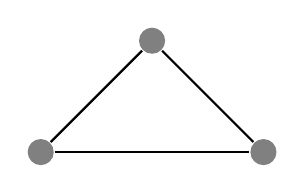
\begin{tikzpicture}[-,>=stealth',auto,node distance=2cm, thick]
  \node (A) [fill=gray, circle, minimum size=.25cm]                   {};
  \node (B) [fill=gray, circle, minimum size=.25cm, below left of=A]  {};
  \node (C) [fill=gray, circle, minimum size=.25cm, below right of=A] {};
  \path (A) edge               (B)
            edge               (C)
        (B) edge               (C);
\end{tikzpicture}
&\quad&
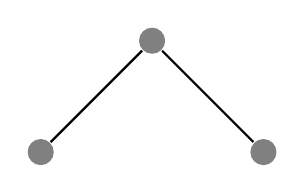
\begin{tikzpicture}[-,>=stealth',auto,node distance=2cm, thick]
  \node (A) [fill=gray, circle, minimum size=.25cm]                   {};
  \node (B) [fill=gray, circle, minimum size=.25cm, below left of=A]  {};
  \node (C) [fill=gray, circle, minimum size=.25cm, below right of=A] {};
  \path (A) edge               (B)
            edge               (C);
\end{tikzpicture}\\
Graph 1 && Graph 2
\end{tabular}
}

\begin{example}
$\forall x \forall y\, (x\neq y \to x\sim y)$ is true for Graph 1 but not Graph 2.
\end{example}
Thus the theory of Graph 1 is different from the theory of Graph 2.

\begin{exercise}
\begin{enumerate}
\item Find a sentence which is true for Graph~2 but not Graph~1.
\item Find a sentence which is true for both graphs.
\end{enumerate}
\end{exercise}

Two finite graphs, $\Gamma$ and $\Gamma'$ are said to be {\em isomorphic} if they have the same number (say $k$) of vertices, and these vertices can be listed as 
\[ v_1,\ldots v_k \mbox { and } v'_1,\ldots v'_k \mbox{ respectively}\]
in such a way that there is an edge from $v_i$ to $v_j$ if and only if there is an edge from $v'_i$ to $v'_j$.

\begin{example}
If $\Gamma$ has three vertices, and every pair of distinct vertices has an edge joining them, then $\Gamma$ is isomorphic to Graph 1.
\end{example}
 
It is intuitively clear that isomorphic graphs have the same theory. The converse is also true.

\begin{theorem}
If two finite graphs have the same theory, they are isomorphic.
\end{theorem}
\begin{proof}
If a graph is finite with $k$ vertices, then there is a sentence $\sigma$ which is true for that graph and says
\begin{quote}
There are exactly $k$ vertices, $x_1,\ldots x_k$, and $x_i\sim x_j$ for all vertices joined by edges, and $\neg x_i\sim x_j$ for all vertices not joined by edges.
\end{quote}
If another graph has the same theory, then $\sigma$ is true for that graph too, so the graphs are isomorphic.
\end{proof}

\subsubsection{Infinite graphs}

It is not true that two infinite graphs which have the same theory must be isomorphic.

Let $T$ be the theory of the infinite (in both directions) graph $\Gamma$ with all vertices of degree 2. 

\begin{center}
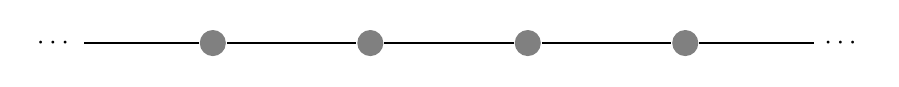
\begin{tikzpicture}[-,>=stealth',auto,node distance=2cm, thick]
  \node (A) [fill=gray, circle, minimum size=.25cm]                   {};
  \node (B) [fill=gray, circle, minimum size=.25cm, right of=A] {};
  \node (C) [fill=gray, circle, minimum size=.25cm, right of=B] {};
  \node (D) [fill=gray, circle, minimum size=.25cm, right of=C] {};  
  \node (AA) [left of=A] {$\cdots$};
  \node (DD) [right of=D] {$\cdots$};
  \path (A) edge               (AA)
            edge               (B)
        (B) edge               (C)
        (C) edge               (D)
        (D) edge               (DD);
\end{tikzpicture}
\end{center}
We will show that $T$ is also the theory another graph, $\Gamma'$, which is not isomorphic to $T$. 

$T$ contains translations of 
\begin{enumerate}
\item There are two vertices not joined by a path of length $\le 2$.
\item There are two vertices not joined by a path of length $\le 3$.
\item There are two vertices not joined by a path of length $\le k$, where $k$ is any fixed number.
\end{enumerate}
The idea is to use the Compactness Theorem to show that $T$ has a model $\Gamma'$ in which there are two fixed vertices not joined by any path at all. Clearly such a $\Gamma'$ cannot be isomorphic to $\Gamma$.

To keep track of the two vertices we give them names. In other  words we add names $a,b$ to our language. The language is now $\{\sim, =, a, b\}$. 

We can now say things like
\begin{enumerate}
\item $\tau_2$: $\exists x\, a\sim x \wedge x\sim b$ ``There is a path of length at most 2 from $a$ to $b$.''
\item $\tau_3$: $\exists x \exists y\, a\sim x \wedge x\sim y \wedge y\sim b$ ``There is a path of length at most 3 from $a$ to $b$.''
\item etc.
\end{enumerate}

Now define
\[S = T\cup\{ \neg\tau_2, \neg \tau_3, \ldots\}.\]
Any finite subset of $S$ has a model consisting of the graph $\Gamma$ with vertices $a$ and $b$ far enough apart. 
\begin{center}
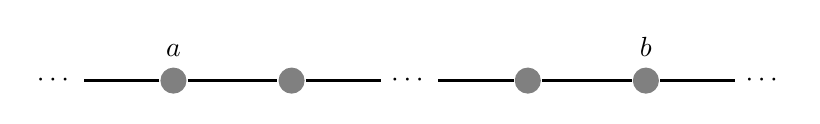
\begin{tikzpicture}[-,>=stealth',auto,node distance=1.5cm, thick]
  \node (A) [fill=gray, circle, minimum size=.25cm]                   [label=above:$a$]{};
  \node (B) [fill=gray, circle, minimum size=.25cm, right of=A] {}; 
  \node (CC) [right of=B]  {$\cdots$};
  \node (C) [fill=gray, circle, minimum size=.25cm, right of=CC] {};
  \node (D) [fill=gray, circle, minimum size=.25cm, right of=C][label=above:$b$] {};  
  \node (AA) [left of=A] {$\cdots$};
  \node (DD) [right of=D] {$\cdots$};
  \path (A) edge               (AA)
            edge               (B)
        (B) edge               (CC)
        (C) edge               (CC)
            edge               (D)
        (D) edge               (DD);
\end{tikzpicture}
\end{center}
So by the Compactness Theorem $S$ has a model, $\Gamma'$, in which $a$ and $b$ are not joined by a path of length $k$ for any $k$. But any two vertices in $\Gamma$ are joined by a path of length $k$ for some $k$. Clearly $\Gamma$ and $\Gamma'$ are not isomorphic.


\section{Arithmetic}

\subsection{The language of arithmetic}

Constant: $0$.

Variables: $x,y,x_0, x_1$, etc.

Function symbols: $s,+,\times$. Instead of $+(x,y)$, we write $(x+y)$ etc.

Predicate: $=$.

The {\em standard interpretation} for the language of arithmetic is 
\begin{enumerate}
\item Domain $N=\{0,1,2,3,\ldots\}$.
\item Extension of the constant $0$ is the integer $0$.
\item Extensions of $+$ and $\times$ are the usual addition and multiplication in $N$.
\item Extension of $s$ is the {\em successor function}: $s0 = 1$, $s1 = 2$, $s2 = 3$, etc.
\end{enumerate}

Notice that each integer in $N$ has a name: $1=s0$, $2=ss0$, $3=sss0$, etc.

\subsection {The axioms of Robinson arithmetic.}

The following sentences are the called the axioms of Robinson arithmetic. We call them ``the Axioms'' for short. 

\begin{description}
\item[Axiom Q1] $\forall x\, \forall y\, (x \neq y \to sx \neq sy)$.
\item[Axiom Q2] $\forall x\, 0\neq sx$.
\item[Axiom Q3] $\forall x\,(x\neq 0\to \exists y\,x=sy)$.
\item[Axiom Q4] $\forall x\,(x + 0) = x$.
\item[Axiom Q5] $\forall x\, \forall y\, (x+sy) = s(x+y)$.
\item[Axiom Q6] $\forall x\,(x \times 0) = 0$.
\item[Axiom Q7] $\forall x\, \forall y\, (x\times sy) = [(x\times y) + x)]$.
\end{description}

From the usual rules of arithmetic which you learned in grade school, you can easily see that the Axioms are all true in the standard interpretation of arithmetic. In other words the standard interpretation is a {\em model} of Robinson arithmetic. Not surprisingly we call the standard interpretation {\em the standard model}. 


\subsection{The theory of Robinson arithmetic}

By definition of ``model'' the Axioms are true in every model (of Robinson arithmetic). The the conclusion of any valid argument whose premises are Axioms, is true in every model. The collection of all these conclusions is {\em the theory of Robinson arithmetic}.

For example $s0\neq ss0$ is a sentence in the theory of Robinson arithmetic because the following argument is valid. 

\centerline{
\begin{tabular}{l}
$\forall x\, \forall y\, (x \neq y \to sx \neq sy)$ (Q1)\\
$\forall x\, 0\neq sx$ (Q2)\\\hline
$s0 \neq ss0$
\end{tabular}}

So $s0 \neq ss0$ in every model.

To check validity of the argument above use a truth tree.

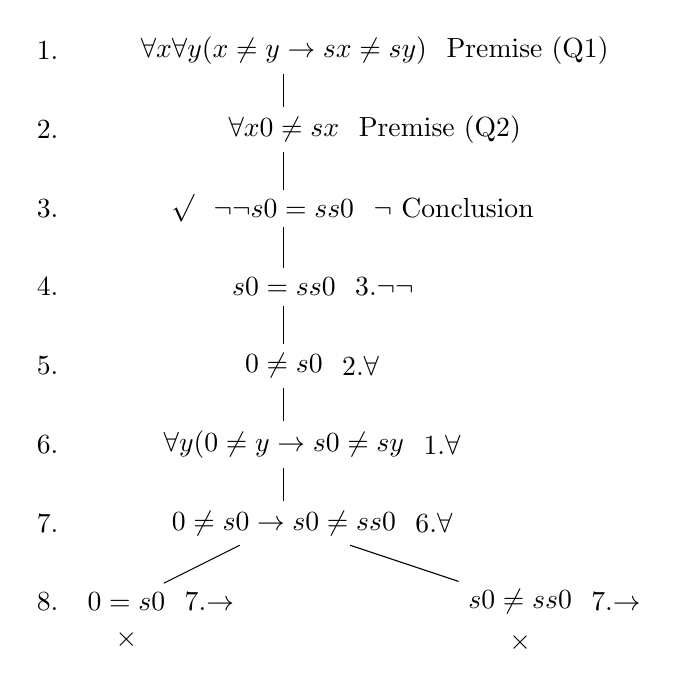
\begin{tikzpicture}
\draw (0,0)      node (11)                       {1.};
\draw (3cm,0)    node (13) [label=right: Premise (Q1)] {$\forall x\forall y  (x\neq y \to sx\neq sy)$};

\draw (0,-1cm)   node (21)                      {2.};
\draw (3cm,-1cm) node (23)  [label=right: Premise (Q2)] {$\forall x 0\neq sx$};
\draw (13) -- (23);

\draw (0,-2cm)   node (31)                     {3.};
\draw (3cm,-2cm) node (33) [label=left:$\surd$] [label=right: $\neg$ Conclusion]   {$\neg\neg s0=ss0 $};
\draw (23) -- (33);

\draw (0,-3cm)   node (41)                     {4.};
\draw (3cm,-3cm) node (43) [label=right:3.$\neg \neg$] {$s0=ss0$};
\draw (33) -- (43);

\draw (0,-4cm)   node (51)                      {5.};
\draw (3cm,-4cm) node (53)  [label=right:2.$\forall$]{$0\neq s0$};
\draw (43) -- (53);

\draw (0,-5cm)   node (61)                      {6.};
\draw (3cm,-5cm) node (63)  [label=right:1.$\forall$] {$\forall y(0\neq y \to s0\neq sy $};
\draw (53) -- (63);

\draw (0,-6cm)   node (71)                      {7.};
\draw (3cm,-6cm) node (73)  [label=right:6.$\forall$] {$0\neq s0 \to s0 \neq ss0$};
\draw (63) -- (73);

\draw (0,-7cm)   node (81)                      {8.};
\draw (1cm,-7cm) node (82) [label=right:7.$\to$] [label=below:$\times$] {$0=s0$};
\draw (6cm,-7cm) node (84) [label=right:7.$\to$] [label=below:$\times$] {$s0 \neq ss0$};
\draw (73) -- (82);
\draw (73) -- (84);

\end{tikzpicture}

\subsection{Pruned truth trees}

From now on we allow shortcuts in truth trees. Axioms do not need to be listed explicitly as premises. Also Lines 3 and 4 in the tree of the previous section can be combined as can Lines 6, 7 and 8. The above truth tree becomes

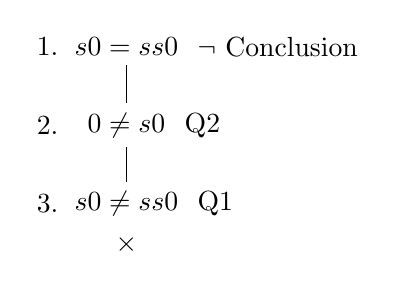
\begin{tikzpicture}
\draw (0cm,0cm)   node (41)                     {1.};
\draw (1cm,0cm) node (43)  [label=right:$\neg$ Conclusion] {$s0=ss0$};
 
\draw (0cm,-1cm)   node (51)                      {2.};
\draw (1cm,-1cm) node (53)  [label=right: Q2] {$0\neq s0$}; 
\draw (43) -- (53);

\draw (0cm,-2cm)   node (61)                      {3.};
\draw (1cm,-2cm) node (63)  [label=right: Q1] [label=below: $\times$]{$s0\neq ss0 $};
\draw (53) -- (63);
\end{tikzpicture}




{\bf Exercise:} Prove that $ss0 \neq sss0$.

{\bf Exercise:} Prove that $sss0 \neq ssss0$.

{\bf Exercise:}  $\underbrace{s\ldots s}_\text{$n$}0\neq\underbrace{s\ldots s}_\text{$n+1$}0$ for all integers $n\ge 0$. Justify this statement.


\subsection{A nonstandard model of Robinson arithmetic}\label{se:nonstandardmodel}

\begin{description}
\item[Domain] $N \cup \{i\}$; we add one new element to $N$.
\item[Extensions] The extension of $0$ is $0$, the same as in the standard model. The extensions of $s,+,\times$ are also same except that we have to define what the successor of $i$ is and how to add and multiply with $i$.
\begin{enumerate}
\item \label{item:successor} $si = i$;
\item \label{item:plus}$x+i = i = i + x$ for all $x$ (including $x=i$);
\item \label{item:times0}$0\times i = 0 = i \times 0$
\item \label{item:times1}$x\times i = i = i \times x$ for all $x\neq 0$.
\end{enumerate}
\end{description}

For example $(3+i)\times(2i)=i\times i = i$. Notice that we do not say anything about subtraction. There is no way to define $i - i$ so that the usual rules of arithmetic hold.

The above interpretation is a model because the Axioms are all true. We check Axioms $Q6$ and $Q7$. The other Axioms are left to the reader.

\begin{description}
\item[Q6] Axiom Q6 is $\forall x\,(x\times 0 = 0)$. We already know $x\times 0 = 0$ for $x$ in $N$, and $i\times 0 = 0$ by Definition~\ref{item:times0} above.

\item[Q7] Axiom Q7 is $\forall x\, \forall y\, [x\times sy = (x\times y + x)]$. We check that both sides of the equation are equal. There are two cases.
\begin{description}
\item[$\mathbf{x=i}$] $x\times sy=i\times sy=i$ because $sy\neq 0$, and $x\times y +x = x\times y + i = i$. 
\item[$\mathbf{y=i}$] $x\times sy=x\times i$, and $x\times y +x = x\times i + x$. If $x=0$, both sides are 0; otherwise both sides equal $i$. 
\end{description}
\end{description}

\subsection{Incompleteness of Robinson arithmetic}

\begin{theorem} $\forall x\, x\neq sx$ is true in the standard model $N$ but not provable from the Axioms. 
\end{theorem}

\begin{proof}
$\forall x\, x \neq sx$ is true because $x\neq x+1$ for all $x$ in $N$. On the other hand $\forall x\, x \neq sx$ is false in the nonstandard model from Section~\ref{se:nonstandardmodel} because $si=i$. If follows that $\forall x\, x \neq sx$ cannot be proved from the Axioms (or else it would be true in all models of Robinson arithmetic).
\end{proof}

\subsection{Induction}

We add a new rule of inference so that we can prove $\forall x\, x \neq sx$. The new rule {\em which works only in the standard model} is
\begin{align*}
\ldots &0 \ldots\\
\underline{\neg \ldots}&\underline{a \ldots}\\ 
\ldots &b \ldots\\
\neg \ldots &sb \ldots
\end{align*}

\begin{example}
We use the new rule to prove  $\forall x\, x \neq sx$ by the method of pruned truth trees.

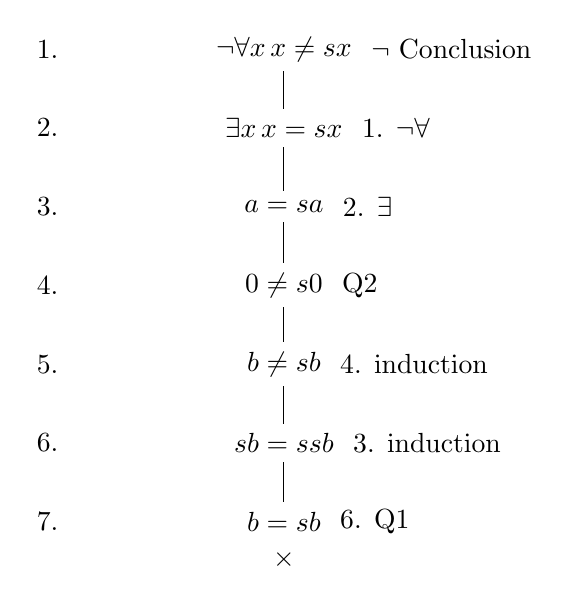
\begin{tikzpicture}
\draw (0,0)      node (11)                       {1.};
\draw (3cm,0)    node (13) [label=right:$\neg$ Conclusion] {$\neg \forall x\, x \neq sx$};

\draw (0,-1cm)   node (21)                      {2.};
\draw (3cm,-1cm) node (23)  [label=right: 1. $\neg\forall$] {$\exists x\, x =sx$};
\draw (13) -- (23);

\draw (0,-2cm)   node (31)                     {3.};
\draw (3cm,-2cm) node (33) [label=right: 2. $\exists$]   {$a=sa$};
\draw (23) -- (33);

\draw (0,-3cm)   node (41)                     {4.};
\draw (3cm,-3cm) node (43) [label=right: Q2] {$0\neq s0$};
\draw (33) -- (43);

\draw (0,-4cm)   node (51)                      {5.};
\draw (3cm,-4cm) node (53)  [label=right:4. induction ]{$b\neq sb$};
\draw (43) -- (53);

\draw (0,-5cm)   node (61)                      {6.};
\draw (3cm,-5cm) node (63)  [label=right:3. induction] {$sb = ssb$};
\draw (53) -- (63);

\draw (0,-6cm)   node (71)                      {7.};
\draw (3cm,-6cm) node (73)  [label=right: {6. Q1}][label=below: {$\times$}] {$b = sb$};
\draw (63) -- (73);

\end{tikzpicture}
\end{example}


\subsection{Induction IRL}

In previous sections we studied the axioms Q1 - Q7 for $N$, and we used induction to prove $\forall x\,x\neq sx$. 
However induction has many applications beyond predicate logic. For those application one uses different notation.

\begin{enumerate}
\item Different letters are used for variables: $m, n, i, j$ instead of $x,y,z$. 
\item Predicates are written as $P_n$ instead of $Px$.
\item One writes $n+1$ instead of $sn$ and 3 instead of $sss0$ etc.
\end{enumerate}

\begin{example}
$P_n$ is the predicate 
$0 +1 + 2 + \cdots + n = \frac{n(n+1)}{2}$.
\end{example}

In addition to this new notation, Q1 - Q7 are not used. Familiarity with the usual rules of arithmetic is assumed, and these rules are used freely.

Finally the rule of induction which we used previously is converted to the so-called agrument by induction. 

\begin{theorem}[Argument by induction]\label{th:induction}
The following argument is valid in $N$.\\
\centerline{
\begin{tabular}{l}
$P_0$\\
$\forall n\, (P_n \to P_{n+1})$\\\hline
$\forall n\, P_n$
\end{tabular}
}
\end{theorem}

{\em Proof.}
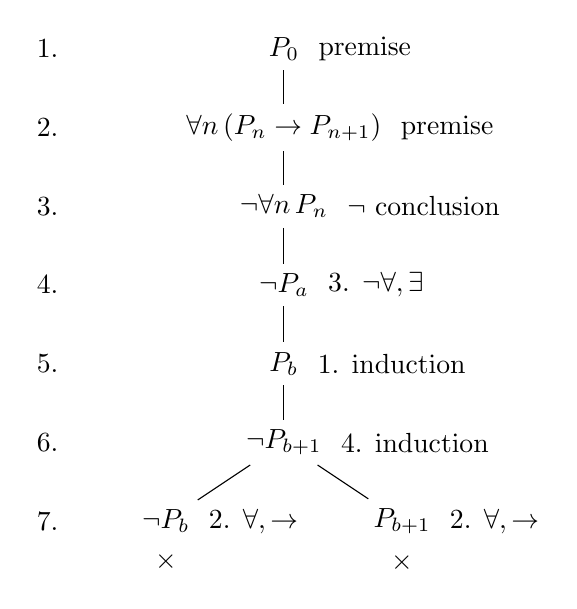
\begin{tikzpicture}[baseline=0in]
\draw (0,0)      node (11)                       {1.};
\draw (3cm,0)    node (13) [label=right:premise] {$P_0$};

\draw (0,-1cm)   node (21)                      {2.};
\draw (3cm,-1cm) node (23)  [label=right:premise] {$\forall n\,(P_n\to P_{n+1})$};
\draw (13) -- (23); 

\draw (0,-2cm)   node (31)                     {3.};
\draw (3cm,-2cm) node (33) [label=right:{$\neg$ conclusion}]   {$\neg\forall n\, P_n$};
\draw (23) -- (33);

\draw (0,-3cm)   node (41)                     {4.};
\draw (3cm,-3cm) node (43) [label=right:{3. $\neg\forall, \exists$}] {$\neg P_a$};
\draw (33) -- (43);

\draw (0,-4cm)   node (51)                      {5.};
\draw (3cm,-4cm) node (53) [label=right:1. induction] {$P_b$};
\draw (43) -- (53);

\draw (0,-5cm)   node (61)                      {6.};
\draw (3cm,-5cm) node (63)    [label=right:{4. induction}] {$\neg P_{b+1}$};
\draw (53) -- (63);

\draw (0,-6cm)   node (71)                       {7.};
\draw (1.5cm,-6cm) node (73) [label=below:$\times$] [label=right:{2. $\forall, \to$}] {$\neg P_{b}$};
\draw (63) -- (73);
\draw (4.5cm,-6cm) node (75)  [label=below:$\times$][label=right:{2. $\forall, \to$}] {$P_{b+1}$};
\draw (63) -- (75);
\end{tikzpicture}\\
\rightline{$\Square$}

A proof by induction consists of verifying the two hypotheses in Theorem~\ref{th:induction}. As an example we prove $\forall n\, P_n$ where $P_n$ is  
\[ 0 + 1 + \cdots + n = \frac{n(n+1)}{2}.\]
{\bf Basis step.} Check that $P_0$ is true:
\[ 0 = \frac{0(0+1)}{2}. \]
{\bf Induction step.} Show that $\forall n\, (P_n \to P_{n+1})$ is true. If $P_n$ is false, then $P_n \to P_{n+1}$ is true, so assume that $P_n$ is true.
\begin{align}
 0 + 1 + \cdots + n =  \frac{n(n+1)}{2}
 &\mbox{\quad because $P_n$ is true}\\
 0 + 1 + \cdots + n + (n+1) =  \frac{n(n+1)}{2}+ (n+1)
  &\mbox{\quad from (1)}\\
\frac{n(n+1)}{2}+ (n+1) = \frac{(n+1)(n+2)}{2} 
&\mbox{\quad details omitted}\\
0 + 1 + \cdots + n + (n+1) = \frac{(n+1)(n+2)}{2}
&\mbox{ \quad from (2) and (3)}
\end{align}
\rightline{$\Square$}


\end{document}
